\section{Resoconto delle attività di verifica}
\subsection{Metriche di qualità di processo}
In questa sezione vengono riportati i risultati dell'attività di verifica effettuata relativa alla qualità del processo.\\
Per calcolare le seguenti misure abbiamo utilizzato le formule e le nozioni descritte nel documento di \textit{Norme di Progetto} e i dati redatti nel documento di \textit{Piano di Progetto}.\\
La metrica di Code Coverage non è stata testata nello sviluppo del PoC in quanto verrà eseguita successivamente in seguito ai Test nel codice del progetto.\\
\begin{longtable}{ 
		>{\centering}M{0.45\textwidth} 
		>{\centering}M{0.17\textwidth}
		>{\centering}M{0.25\textwidth} 
		}
	\rowcolorhead
	\headertitle{Metrica} &
	\centering \headertitle{Valore} &	
	\headertitle{Esito} 
	\endfirsthead	
	\endhead
	
	Planned Value & 8784,29 \euro & Superato\tabularnewline
	Actual Cost & 7460 \euro & Superato\tabularnewline
	Estimated at Completion & 12944,93 \euro & Superato\tabularnewline
	Earned Value & 8490,07 \euro & Superato\tabularnewline
	Estimated to Complete & 5484,93 \euro & Superato\tabularnewline
	Cost Variance& 1030,07 \euro & Superato\tabularnewline
	Schedule Variance & -3,46\% & Superato\tabularnewline
	Budget Variance & 1324,29 \euro & Superato\tabularnewline
	Requirement Stability Index& 100\% & Superato\tabularnewline
	Code coverage & - & Non testato\tabularnewline
	Rischi non previsti & 0 & Superato\tabularnewline
	Metriche soddisfatte & 80,95\% & Superato\tabularnewline
\end{longtable}
\noindent Qui vengono riportati i grafici per varie metriche di processo significative nei tre periodi identificati.
Nei primi tre grafici viene rappresentato di quanto differisce ciascun valore da quello precedente per periodo.
\paragraph{Planned Value}
\begin{center}
\begin{figure}[H]
  \centering
  \renewcommand{\thefigure}{1}
  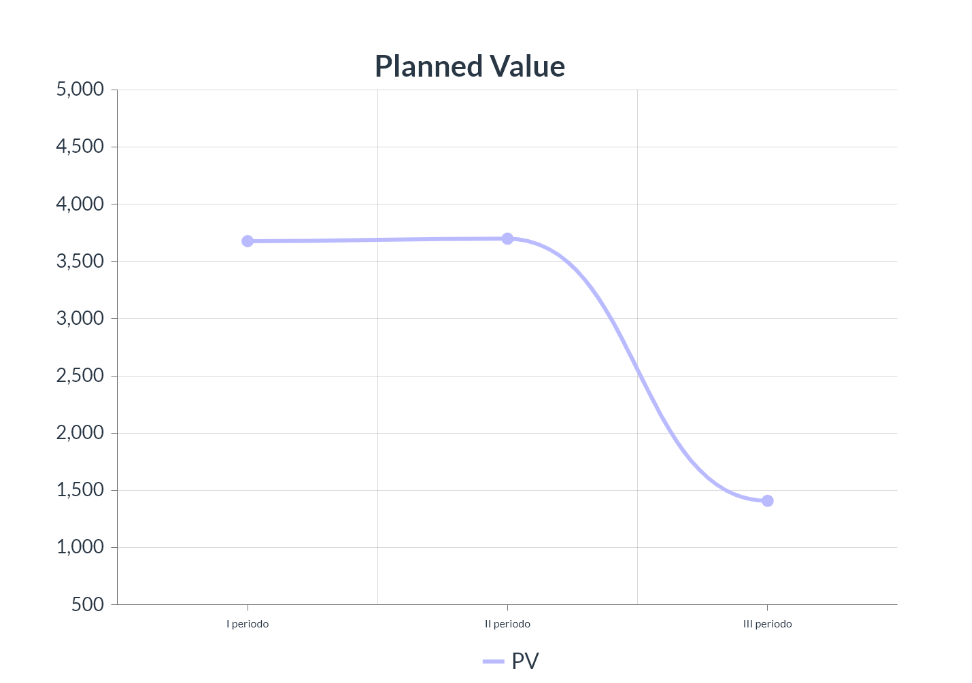
\includegraphics[width=10cm]{./res/images/PVGraph.png}
  \caption{Planned Value}
  \label{fig:Grafico Planned Value}
\end{figure}
\end{center}
\pagebreak
\paragraph{Actual Cost}
\begin{center}
\begin{figure}[H]
  \centering
  \renewcommand{\thefigure}{2}
  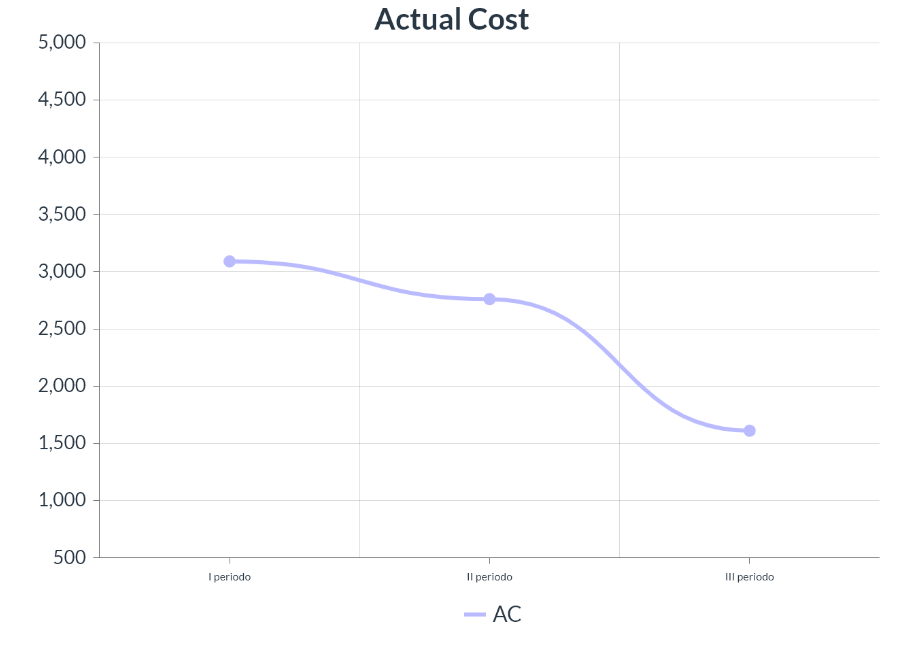
\includegraphics[width=10cm]{./res/images/ACGraph.png}
  \caption{Actual Cost}
  \label{fig:Grafico Actual Cost}
\end{figure}
\end{center}
\paragraph{Earned Value}
\begin{center}
\begin{figure}[H]
  \centering
  \renewcommand{\thefigure}{3}
  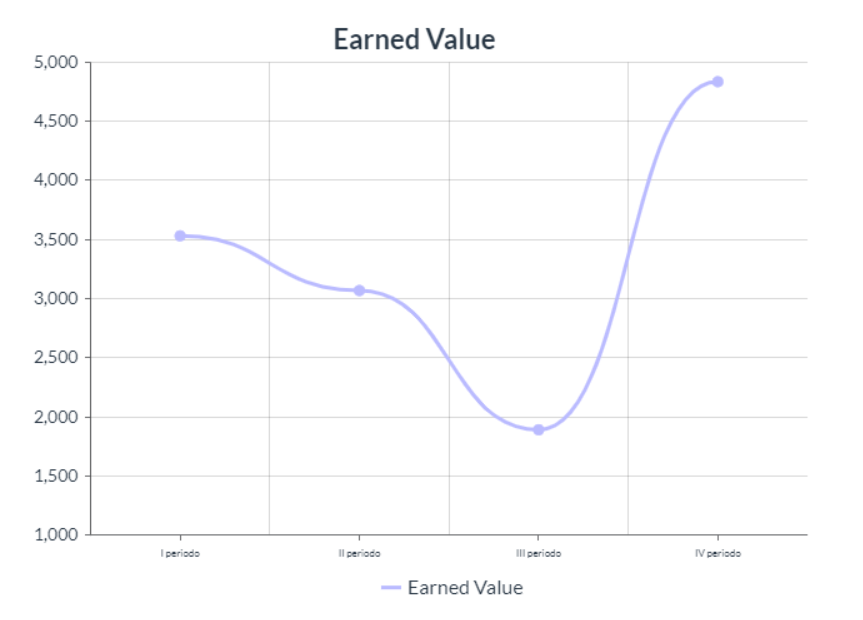
\includegraphics[width=10cm]{./res/images/EVGraph.png}
  \caption{Earned Value}
  \label{fig:Grafico Earned Value}
\end{figure}
\end{center}
\pagebreak
\paragraph{Cost Variance}
\begin{center}
\begin{figure}[H]
  \centering
  \renewcommand{\thefigure}{4}
  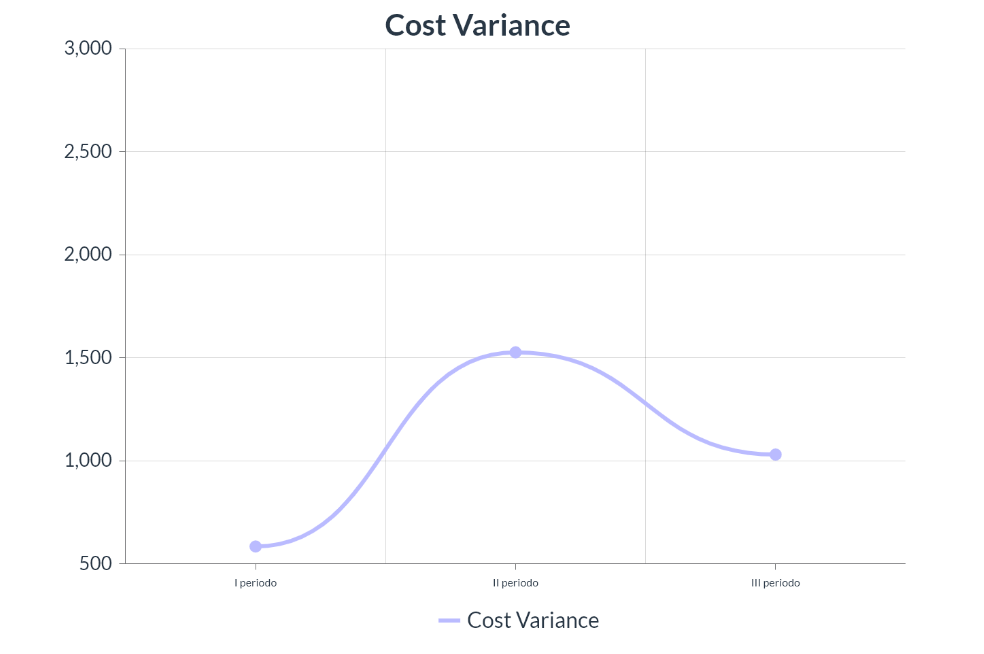
\includegraphics[width=10cm]{./res/images/CVGraph.png}
  \caption{Cost Variance}
  \label{fig:Grafico Cost Variance}
\end{figure}
\end{center}

\paragraph{Schedule Variance}
\begin{center}
\begin{figure}[H]
  \centering
  \renewcommand{\thefigure}{5}
  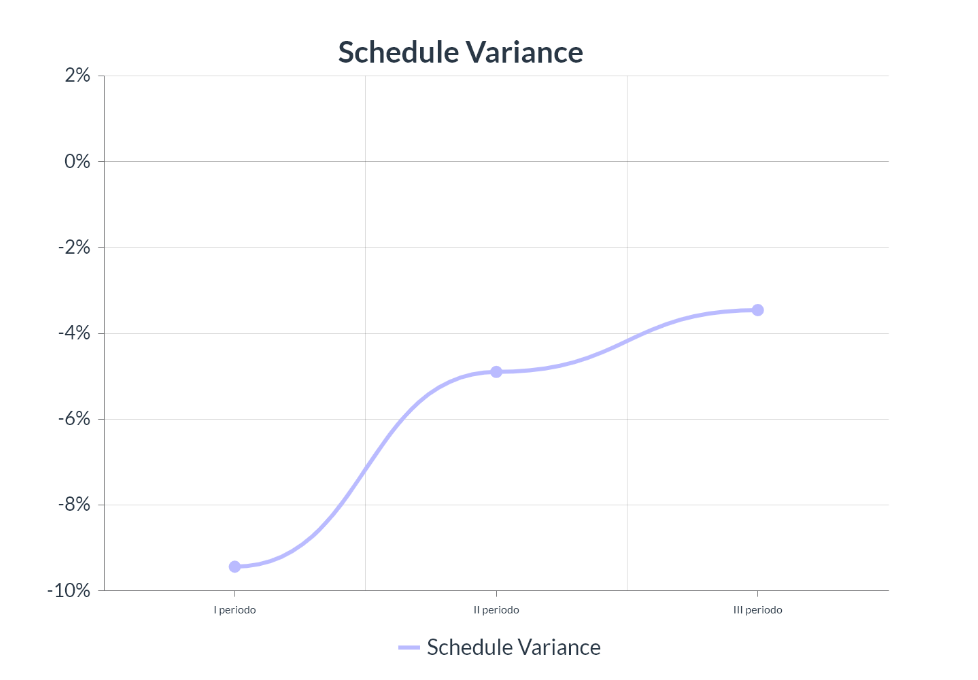
\includegraphics[width=10cm]{./res/images/SVGraph.png}
  \caption{Schedule Variance}
  \label{fig:Grafico Schedule Variance}
\end{figure}
\end{center}
\pagebreak
\paragraph{Budget Variance}
\begin{center}
\begin{figure}[H]
  \centering
  \renewcommand{\thefigure}{6}
  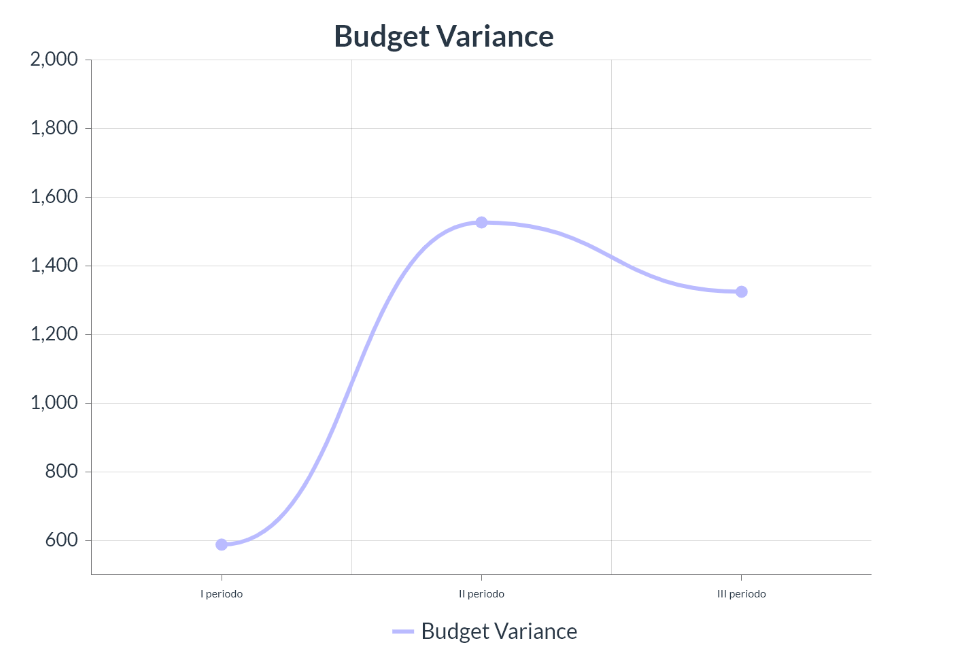
\includegraphics[width=10cm]{./res/images/BVGraph.png}
  \caption{Budget Variance}
  \label{fig:Grafico Budget Variance}
\end{figure}
\end{center}

\subsubsection{Indice di Gulpease}
\noindent Nella seguente tabella vengono riportati gli indici di Gulpease calcolati sulle ultime versioni dei seguenti documenti.\\
Per calcolare i seguenti valori non sono stati considerati: i changelog, la pagina di introduzione del documento, l'indice, tabelle con valori, intestazioni a piè di pagina, captions e la sezione di "Informazioni generali" nei verbali. Sono state incluse invece le colonne di tabelle contenenti descrizioni significative e gli elenchi puntati che contenevano frasi significative. 
\begin{longtable}{ 
		>{\centering}M{0.45\textwidth} 
		>{\centering}M{0.17\textwidth}
		>{\centering}M{0.25\textwidth} 
		}
	\rowcolorhead
	\headertitle{Documento} &
	\centering \headertitle{Valore} &	
	\headertitle{Esito} 
	\endfirsthead	
	\endhead
	
	Analisi dei requisiti & 80 & Superato\tabularnewline
	Glossario & 74 & Superato\tabularnewline
	Norme di progetto & 73 & Superato\tabularnewline
	Piano di progetto & 67 & Superato\tabularnewline
	Piano di qualifica & 72 & Superato\tabularnewline
	Studio di fattibilità & 80 & Superato\tabularnewline
	VE 22-10-25 & 82 & Superato\tabularnewline
	VE 22-10-26 & 84 & Superato\tabularnewline
	VE 22-11-17	& 75 & Superato\tabularnewline
	VE 23-01-11	& 57 & Superato\tabularnewline
	VE 23-01-18	& 69 & Superato\tabularnewline
	VE 23-02-17 & 70 & Superato\tabularnewline
	VI 22-10-25 & 74 & Superato\tabularnewline
	VI 22-10-26 & 79 & Superato\tabularnewline
	VI 22-11-04 & 63 & Superato\tabularnewline
	VI 22-11-09 & 88 & Superato\tabularnewline
	VI 22-11-16 & 63 & Superato\tabularnewline
	VI 22-11-23 & 72 & Superato\tabularnewline
	VI 22-12-01 & 60 & Superato\tabularnewline
	VI 22-12-07 & 78 & Superato\tabularnewline
	VI 22-12-14 & 69 & Superato\tabularnewline
	VI 23-01-04 & 63 & Superato\tabularnewline
	VI 23-01-25 & 68 & Superato\tabularnewline
	VI 23-02-01 & 65 & Superato\tabularnewline
	VI 23-02-08 & 58 & Superato\tabularnewline
	VI 23-02-24 & 68 & Superato\tabularnewline
	VI 23-02-28 & 65 & Superato\tabularnewline
	VI 23-03-16 & 67 & Superato\tabularnewline
	
	
\end{longtable}

\begin{center}
\begin{figure}[H]
  \centering
  \renewcommand{\thefigure}{7}
  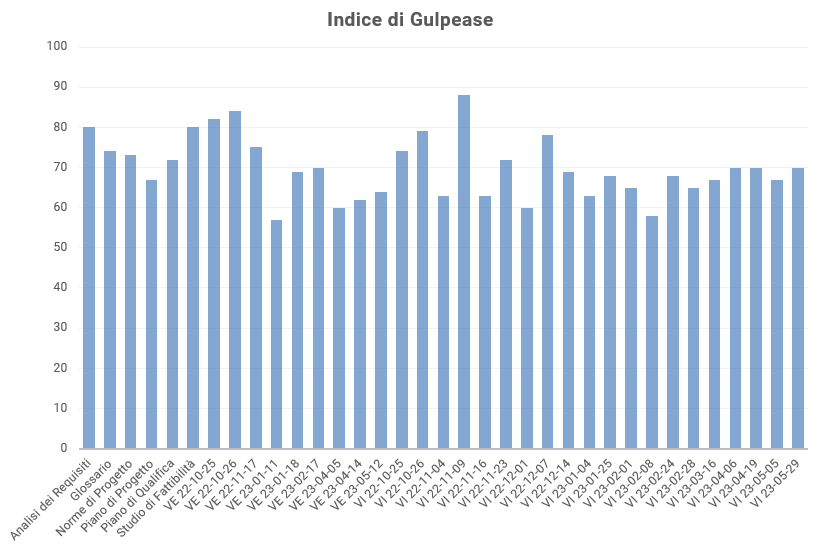
\includegraphics[width=10cm]{./res/images/GulpeaseGen.png}
  \caption{Indice di Gulpease dei documenti}
  \label{fig:Indice di Gulpease dei documenti}
\end{figure}
\end{center}
\pagebreak
\noindent Qui ora vengono riportati i grafici che analizzano l'andamento dell'indice di Gulpease di documenti in continua evoluzione.
\paragraph{Indice di Gulpease - Analisi dei Requisiti}
\begin{center}
\begin{figure}[H]
  \centering
  \renewcommand{\thefigure}{8}
  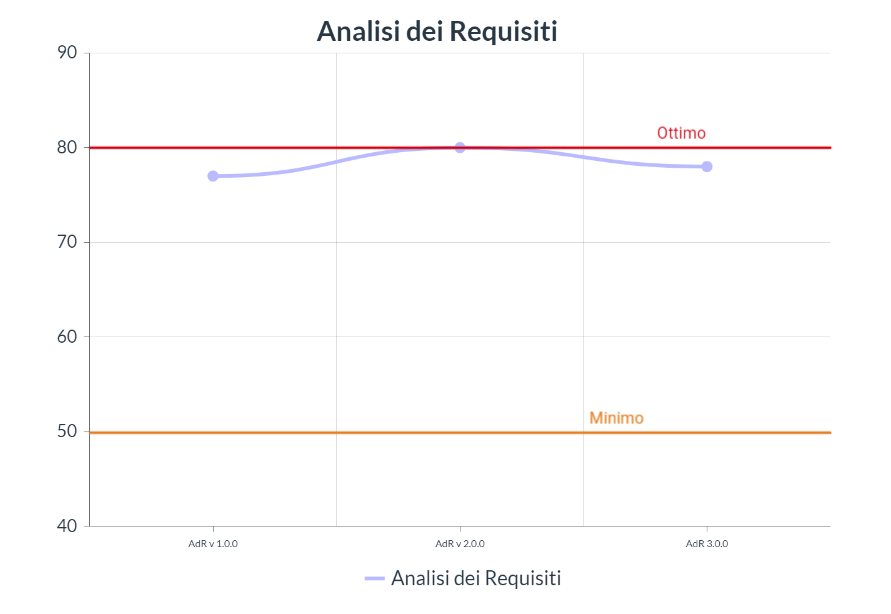
\includegraphics[width=10cm]{./res/images/AdRGraph.png}
  \caption{Indice di Gulpease - Analisi dei Requisiti}
  \label{fig:Indice di Gulpease - Analisi dei Requisiti}
\end{figure}
\end{center}
\pagebreak
\paragraph{Indice di Gulpease - Norme di Progetto}
\begin{center}
\begin{figure}[H]
  \centering
  \renewcommand{\thefigure}{9}
  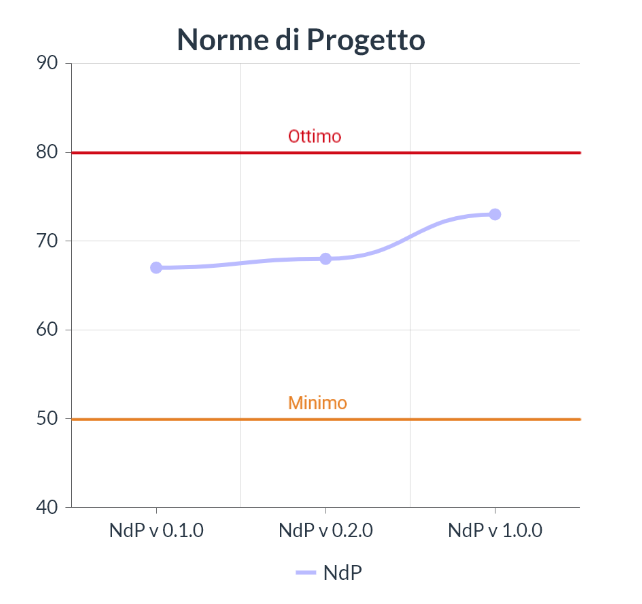
\includegraphics[width=10cm]{./res/images/NdPGraph.png}
  \caption{Indice di Gulpease - Norme di Progetto}
  \label{fig:Indice di Gulpease - Norme di Progetto}
\end{figure}
\end{center}
\pagebreak
\paragraph{Indice di Gulpease - Piano di Progetto}
\begin{center}
\begin{figure}[H]
  \centering
  \renewcommand{\thefigure}{10}
  \includegraphics[width=10cm]{./res/images/PdPGraph.png}
  \caption{Indice di Gulpease - Piano di Progetto}
  \label{fig:Indice di Gulpease - Piano di Progetto}
\end{figure}
\end{center}
\pagebreak
\paragraph{Indice di Gulpease - Piano di Qualifica}
\begin{center}
\begin{figure}[H]
  \centering
  \renewcommand{\thefigure}{11}
  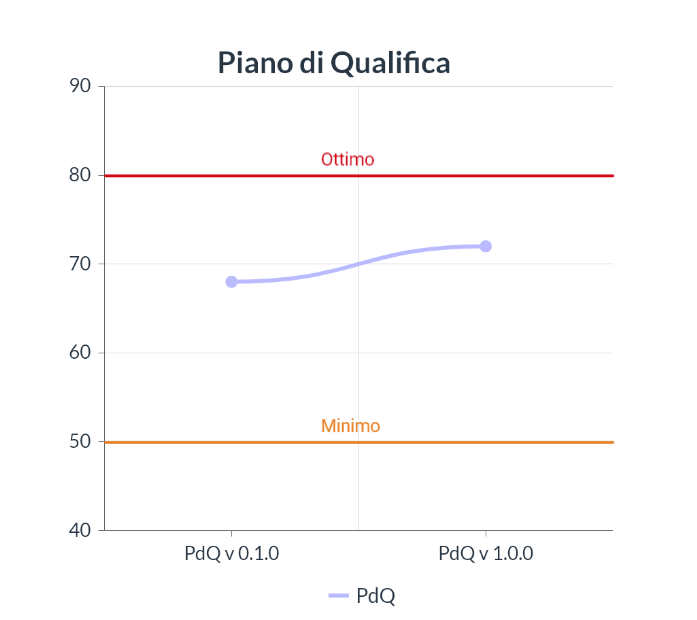
\includegraphics[width=10cm]{./res/images/PdQGraph.png}
  \caption{Indice di Gulpease - Piano di Qualifica}
  \label{fig:Indice di Gulpease - Piano di Qualifica}
\end{figure}
\end{center}

\subsection{Metriche di qualità del prodotto}
In questa sezione vengono riportati i risultati dell'attività di verifica effettuata relativa alla qualità del prodotto, nel contesto del PoC.\\
La metrica di Percentuale di requisiti soddisfatti non è stata testata in quanto non siamo ancora nella fase di Codifica.

\begin{longtable}{ 
		>{\centering}M{0.45\textwidth} 
		>{\centering}M{0.17\textwidth}
		>{\centering}M{0.25\textwidth} 
		}
	\rowcolorhead
	\headertitle{Metrica} &
	\centering \headertitle{Valore} &	
	\headertitle{Esito} 
	\endfirsthead	
	\endhead
	Percentuale di requisiti soddisfatti& - & Non testato\tabularnewline
	Densità di fallimenti durante l'esecuzione& 0\% & Superato\tabularnewline
	Tempo medio di risposta & minore di 1s & Superato\tabularnewline
	Tempo di caricamento& 7 secondi & Superato\tabularnewline
	Facilità di apprendimento& 90 secondi & Superato\tabularnewline
	Densità dei commenti & 15,93\% & Superato\tabularnewline
	Browser supportati & 100\% & Superato\tabularnewline
\end{longtable}
\noindent Nella seguente tabella è stata calcolata la Complessità Ciclomatica del PoC.
\begin{longtable}{ 
		>{\centering}M{0.40\textwidth} 
		>{\centering}M{0.15\textwidth}
		>{\centering}M{0.20\textwidth}
		}
	\rowcolorhead
	\headertitle{Modulo} &
	\headertitle{Valore} &
	\headertitle{Esito} 	
	\endfirsthead	
	\endhead
	Player.js & 2 & Superato\tabularnewline
	Light.js & 1 & Superato\tabularnewline
	Product.js & 1 & Superato\tabularnewline
	Raycasting.js & 6 & Superato\tabularnewline
	Renderer.js & 2 & Superato\tabularnewline
	Showroom\_poc.js & 1 & Superato\tabularnewline
	Source\_loader.js & 2 & Superato\tabularnewline
	UI\_listeners.js & 1 & Superato\tabularnewline
	
\end{longtable}

Il PoC è stato testato sui seguenti browser:
\begin{longtable}{ 
		>{\centering}M{0.45\textwidth} 
		>{\centering}M{0.25\textwidth} 
		}
	\rowcolorhead
	\headertitle{Browser} &
	\headertitle{Esito} 
	\endfirsthead	
	\endhead
	
	Google Chrome (versione $ \ge 110 $) & Supportato\tabularnewline
	Microsoft Edge (versione $ \ge 110 $) & Supportato\tabularnewline
	Mozilla Firefox (versione $ \ge 109 $) & Supportato\tabularnewline
	Safari (versione $ \ge 16 $) & Supportato\tabularnewline
	Opera (versione $ \ge 95 $) & Supportato\tabularnewline

\end{longtable}
